\documentclass[11pt]{article}

\usepackage{times}
\usepackage{epsf}
\usepackage{epsfig}
\usepackage{amsmath, alltt, amssymb, xspace}
\usepackage{wrapfig}
\usepackage{fancyhdr}
\usepackage{url}
\usepackage{verbatim}
\usepackage{fancyvrb}

\usepackage{subfigure}
\usepackage{cite}
%\usepackage{cases}
%\usepackage{ltexpprt}
%\usepackage{verbatim}

%\topmargin      -0.70in  % distance to headers
%\headheight     0.2in   % height of header box
%\headsep        0.4in   % distance to top line
%\footskip       0.3in   % distance from bottom line

% Horizontal alignment
\topmargin      -0.50in  % distance to headers
\oddsidemargin  0.0in
\evensidemargin 0.0in
\textwidth      6.5in
\textheight     8.9in 


%\centerfigcaptionstrue

%\def\baselinestretch{0.95}


\newcommand\discuss[1]{\{\textbf{Discuss:} \textit{#1}\}}
%\newcommand\todo[1]{\vspace{0.1in}\{\textbf{Todo:} \textit{#1}\}\vspace{0.1in}}
\newtheorem{problem}{Problem}[section]
%\newtheorem{theorem}{Theorem}
%\newtheorem{fact}{Fact}
\newtheorem{define}{Definition}[section]
%\newtheorem{analysis}{Analysis}
\newcommand\vspacenoindent{\vspace{0.1in} \noindent}

%\newenvironment{proof}{\noindent {\bf Proof}.}{\hspace*{\fill}~\mbox{\rule[0pt]{1.3ex}{1.3ex}}}
%\newcommand\todo[1]{\vspace{0.1in}\{\textbf{Todo:} \textit{#1}\}\vspace{0.1in}}

%\newcommand\reducespace{\vspace{-0.1in}}
% reduce the space between lines
%\def\baselinestretch{0.95}

\newcommand{\fixmefn}[1]{ \footnote{\sf\ \ \fbox{FIXME} #1} }
\newcommand{\todo}[1]{
\vspace{0.1in}
\fbox{\parbox{6in}{TODO: #1}}
\vspace{0.1in}
}

\newcommand{\mybox}[1]{
\vspace{0.2in}
\noindent
\fbox{\parbox{6.5in}{#1}}
\vspace{0.1in}
}


\newcounter{question}
\setcounter{question}{1}

\newcommand{\myquestion} {{\vspace{0.1in} \noindent \bf Question \arabic{question}:} \addtocounter{question}{1} \,}

\newcommand{\myproblem} {{\noindent \bf Problem \arabic{question}:} \addtocounter{question}{1} \,}


\newcommand{\copyrightnoticeA}[1]{
\vspace{0.1in}
\fbox{\parbox{6in}{\small Copyright \copyright\ 2006 - 2014\ \ Wenliang Du, Syracuse University.\\ 
      The development of this document is partially funded by 
      the National Science Foundation's Course, Curriculum, and Laboratory 
      Improvement (CCLI) program under Award No. 0618680 and 0231122. 
      Permission is granted to copy, distribute and/or modify this document
      under the terms of the GNU Free Documentation License, Version 1.2
      or any later version published by the Free Software Foundation.
      A copy of the license can be found at http://www.gnu.org/licenses/fdl.html.}}
\vspace{0.1in}
}


\newcommand{\copyrightnotice}[1]{
\vspace{0.1in}
\fbox{\parbox{6in}{\small Copyright \copyright\ 2006 - 2014\ \ Wenliang Du, Syracuse University.\\
      The development of this document is/was funded by three grants from
      the US National Science Foundation: Awards No. 0231122 and 0618680 from
      TUES/CCLI and  Award No. 1017771 from Trustworthy Computing.
      This lab was imported into the Labtainer framework by the Naval Postgraduate 
      School, Center for Cybersecurity and Cyber Operations under National Science 
      Foundation Award No. 1438893.
      Permission is granted to copy, distribute and/or modify this document
      under the terms of the GNU Free Documentation License, Version 1.2
      or any later version published by the Free Software Foundation.
      A copy of the license can be found at http://www.gnu.org/licenses/fdl.html.}}
\vspace{0.1in}
}

\newcommand{\copyrightnoticeB}[1]{
\vspace{0.1in}
\fbox{\parbox{6in}{\small Copyright \copyright\ 2006 - 2014\ \ Wenliang Du, Syracuse University.\\
      The development of this document is/was funded by the following grants from
      the US National Science Foundation: No. 0231122, 0618680, and 1303306.
      Permission is granted to copy, distribute and/or modify this document
      under the terms of the GNU Free Documentation License, Version 1.2
      or any later version published by the Free Software Foundation.
      A copy of the license can be found at http://www.gnu.org/licenses/fdl.html.}}
\vspace{0.1in}
}


\newcommand{\nocopyrightnotice}[1]{
\vspace{0.1in}
\fbox{\parbox{6in}{\small  
      The development of this document is funded by 
      the National Science Foundation's Course, Curriculum, and Laboratory 
      Improvement (CCLI) program under Award No. 0618680 and 0231122. 
      Permission is granted to copy, distribute and/or modify this document.
      }}
\vspace{0.1in}
}

\newcommand{\idea}[1]{
\vspace{0.1in}
{\sf IDEA:\ \ \fbox{\parbox{5in}{#1}}}
\vspace{0.1in}
}

\newcommand{\questionblock}[1]{
\vspace{0.1in}
\fbox{\parbox{6in}{#1}}
\vspace{0.1in}
}


\newcommand{\minix}{{\tt Minix}\xspace}
\newcommand{\unix}{{\tt Unix}\xspace}
\newcommand{\linux}{{\tt Linux}\xspace}
\newcommand{\ubuntu}{{\tt Ubuntu}\xspace}
\newcommand{\selinux}{{\tt SELinux}\xspace}
\newcommand{\freebsd}{{\tt FreeBSD}\xspace}
\newcommand{\solaris}{{\tt Solaris}\xspace}
\newcommand{\windowsnt}{{\tt Windows NT}\xspace}
\newcommand{\setuid}{{\tt Set-UID}\xspace}
%\newcommand{\smx}{{\tt Smx}\xspace}
\newcommand{\smx}{{\tt Minix}\xspace}
\newcommand{\relay}{{\tt relay}\xspace}
\newcommand{\isys}{{\tt iSYS}\xspace}
\newcommand{\ilan}{{\tt iLAN}\xspace}
\newcommand{\iSYS}{{\tt iSYS}\xspace}
\newcommand{\iLAN}{{\tt iLAN}\xspace}
\newcommand{\iLANs}{{\tt iLAN}s\xspace}
\newcommand{\bochs}{{\tt Bochs}\xspace}

\newcommand\FF{{\mathcal{F}}}

\newcommand{\argmax}[1]{
\begin{minipage}[t]{1.25cm}\parskip-1ex\begin{center}
argmax
#1
\end{center}\end{minipage}
\;
}

\newcommand{\bm}{\boldmath}
\newcommand  {\bx}    {\mbox{\boldmath $x$}}
\newcommand  {\by}    {\mbox{\boldmath $y$}}
\newcommand  {\br}    {\mbox{\boldmath $r$}}


%\pagestyle{fancyplain}
%\lhead[\thepage]{\thesection}      % Note the different brackets!
%\rhead[\thesection]{SEED Laboratories}
%\lfoot[\fancyplain{}{}]{Syracuse University} 
%\cfoot[\fancyplain{}{}]{\thepage} 

\newcommand{\tstamp}{\today}   
%\lhead[\fancyplain{}{\thepage}]         {\fancyplain{}{\rightmark}}
%\chead[\fancyplain{}{}]                 {\fancyplain{}{}}
%\rhead[\fancyplain{}{\rightmark}]       {\fancyplain{}{\thepage}}
%\lfoot[\fancyplain{}{}]                 {\fancyplain{\tstamp}{\tstamp}}
%\cfoot[\fancyplain{\thepage}{}]         {\fancyplain{\thepage}{}}
%\rfoot[\fancyplain{\tstamp} {\tstamp}]  {\fancyplain{}{}}

\pagestyle{fancy}
%\lhead{\bfseries Computer Security Course Project}
\lhead{\bfseries SEED Labs}
\chead{}
\rhead{\small \thepage}
\lfoot{}
\cfoot{}
\rfoot{}

\usepackage{listings}
\usepackage{color}

\definecolor{dkgreen}{rgb}{0,0.6,0}
\definecolor{gray}{rgb}{0.5,0.5,0.5}
\definecolor{mauve}{rgb}{0.58,0,0.82}

\lstset{frame=tb,
  language=C,
  aboveskip=3mm,
  belowskip=3mm,
  showstringspaces=false,
  columns=flexible,
  basicstyle={\small\ttfamily},
  numbers=none,
  numberstyle=\tiny\color{gray},
  keywordstyle=\color{blue},
  commentstyle=\color{dkgreen},
  stringstyle=\color{mauve},
  breaklines=true,
  breakatwhitespace=true,
  tabsize=3
}



\begin{document}

\begin{center}
{\LARGE SSL}
\vspace{0.1in}\\
\end{center}

\copyrightnotice

\section{Overview}
This lab illustrates the use of LDAP to authenticate users of Linux systems,
such that multiple computers share a single repository of user and group information, including
the passwords that authenticate users.  This strategy allows users and administrators
to manage a single set of credentials that can then be used to access multiple computers. 

\subsection {Background}
The student is expect to have separately learned about the basic elements of Linux
users, groups and authentication, e.g., the /etc/passwd and /etc/shadow files.  
The student is also expected to have a basic knowledge of the use of Lightweight Directory
Access Protocol (LDAP).

The student is expected to have some familiarity with the Linux command line,
the basics of the file system, and the ability to located and edit a file.  And some
experience with the Wireshark tool is expected (e.g., the wireshark-intro lab).

\section{Lab Environment}
This lab runs in the Labtainer framework,
available at http://my.nps.edu/web/c3o/labtainers.
That site includes links to a pre-built virtual machine
that has Labtainers installed, however Labtainers can
be run on any Linux host that supports Docker containers.

From your labtainer-student directory start the lab using:
\begin{verbatim}
    labtainer ldap
\end{verbatim}
\noindent A link to this lab manual will be displayed.  


\section{Network Configuration}
This lab includes a client computer, two servers and
an ldap server shown in Figure~\ref{fig:topology}.
When the lab starts, you will get one virtual terminal connected 
to the client, and one connected to the ldap server.

The host names of each component are per the diagram.  The /etc/hosts files
allow use of these host names instead of explicit ip addresses.

The two Linux servers have been configured to use the ldap server to 
authenticate users.  The ldap server has been initially configured
with a single user whose ID is "mike".

The ldap server is configured for the ``example.com'' domain, with
an ldap administrator of ``admin'' whose password is ``adminpass''

\begin{figure}[htb]
\begin{center}
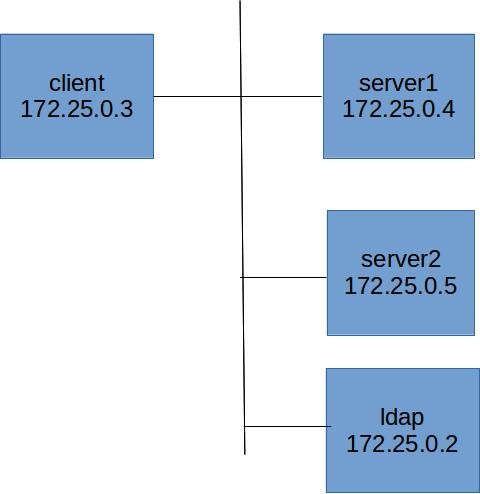
\includegraphics [width=0.8\textwidth,natwidth=621,natheight=403]{ldap.jpg}
\end{center}
\caption{Network topology for the LDAP lab}
\label{fig:topology}
\end{figure}

\section{Lab Tasks}
\subsection{Explore}
On the ldap server, display the ldap directory content using:
\begin{verbatim}
   ldapsearch -x | less
\end{verbatim}
\noindent and observe the entries in the directory. Note entry for ``mike'' and
``projx''.

Start wireshark on the ldap component so that you can observe the protocol traffic.
\begin{verbatim}
   wireshark &
\end{verbatim}
\noindent Select the {\tt eth0} device.
From the ``client'' computer, ssh to server1 as user ``mike'':
\begin{verbatim}
   ssh mike@server1
\end{verbatim}
The initial password for ``mike'' is ``password123''.  The system will require that
your change this password and then you will need to ssh again into server1.  Change
the password to whatever you like, but remember it. Use {\tt ssh} again to login to server1
as mike, providing your new password. Use the {\tt id} command to view your user ID
and group. Then,  view the /etc/passwd file.  Do you see entries
for your user or group?

\subsection{View protocol traffic}
Go to the wireshark window, and stop capturing packets (e.g., the red stop button).
Enter a display filter of ``ldap'', i.e., near the top where it says "Apply a display filter...".
Review the LDAP traffic.  Which components are exchanging packets?  Locate the packet that changed
mike's password and use {\tt File / Export Specified Packets} to save that packet in a file named
{\tt password.pcapng}

\subsection{Use the mike credentials to access another server}
Exit your ssh session from server1.  Then ssh to server2:
\begin{verbatim}
   ssh mike@server2
\end{verbatim}
\noindent What password do you expect to use to authenticate to server2?
After logging into server2, exit that ssh session.

\subsection{Add an LDAP user}
Go to the ldap virtual terminal and use {\tt ls} to see a directory listing.
View the file named {\tt mike.ldif}, it was used to define the user named ``mike''.
Then view the projx.ldif file.
The LDAP command that was used to add the entry defined in mike.ldif is:
\begin{verbatim}
ldapadd -x -W -D "cn=admin,dc=example,dc=com" -f mike.ldif
\end{verbatim}
\noindent Note how the {\tt -D} option names the administrator on whose behalf the
LDAP addition is to be made.  Use {\tt man ldapadd} to learn more about the syntax of
that command. 
The initial password for the mike user was created with this command:
\begin{verbatim}
ldappasswd -s password123 -W -D "cn=admin,dc=example,dc=com" -x "uid=mike,ou=users,dc=example,dc=com"
\end{verbatim}

Create ldif files to define a new group named ``qa'' and a new user having an ID of ``mary''.
Assign mary to the qa group. Take care to adjust the uidNumber and gidNumber values.
Use the ldapadd command to add the new group and the new user.  Use the ldappasswd command to
assign an initial password to mary.  Again, the password for the LDAP administrator is ``adminpass''.

Then go to the client computer and test your ability to ssh as mary to both server1 and server2.

\section{Submission}
After finishing the lab, go to the terminal on your Linux system that was used to start the lab and type:
\begin{verbatim}
    stoplab 
\end{verbatim}
When you stop the lab, the system will display a path to the zipped lab results on your Linux system.  Provide that file to 
your instructor, e.g., via the Sakai site.

\end{document}
